\section{Taxonomy}

\begin{figure}[h] 
    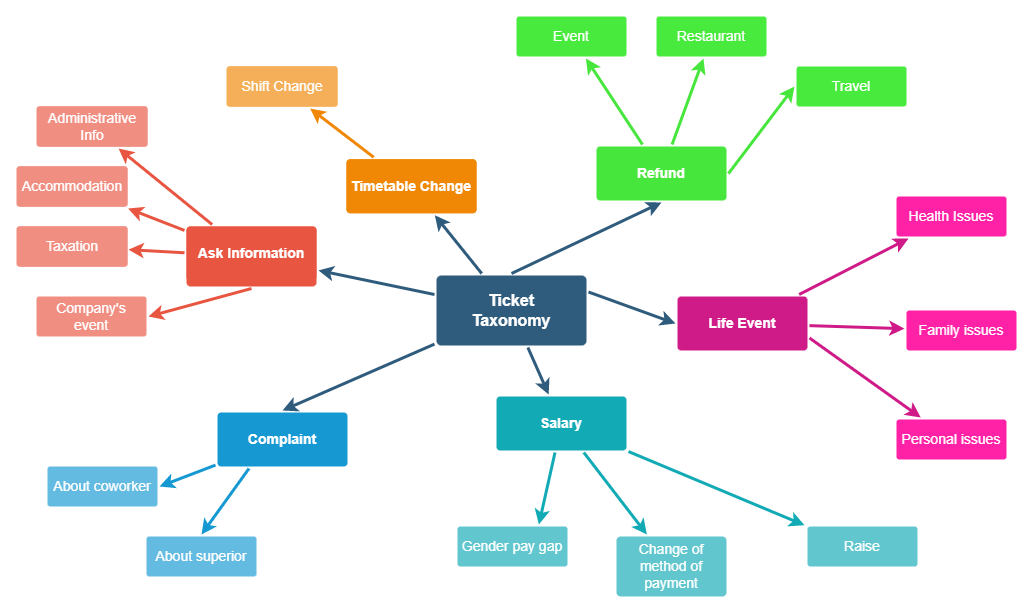
\includegraphics[width=\textwidth]{images/Taxonomy_Tickets.drawio.png}
    \caption{Initial Taxonomy}
    \label{fig:taxonomy}
\end{figure}    

\begin{figure}[h] 
    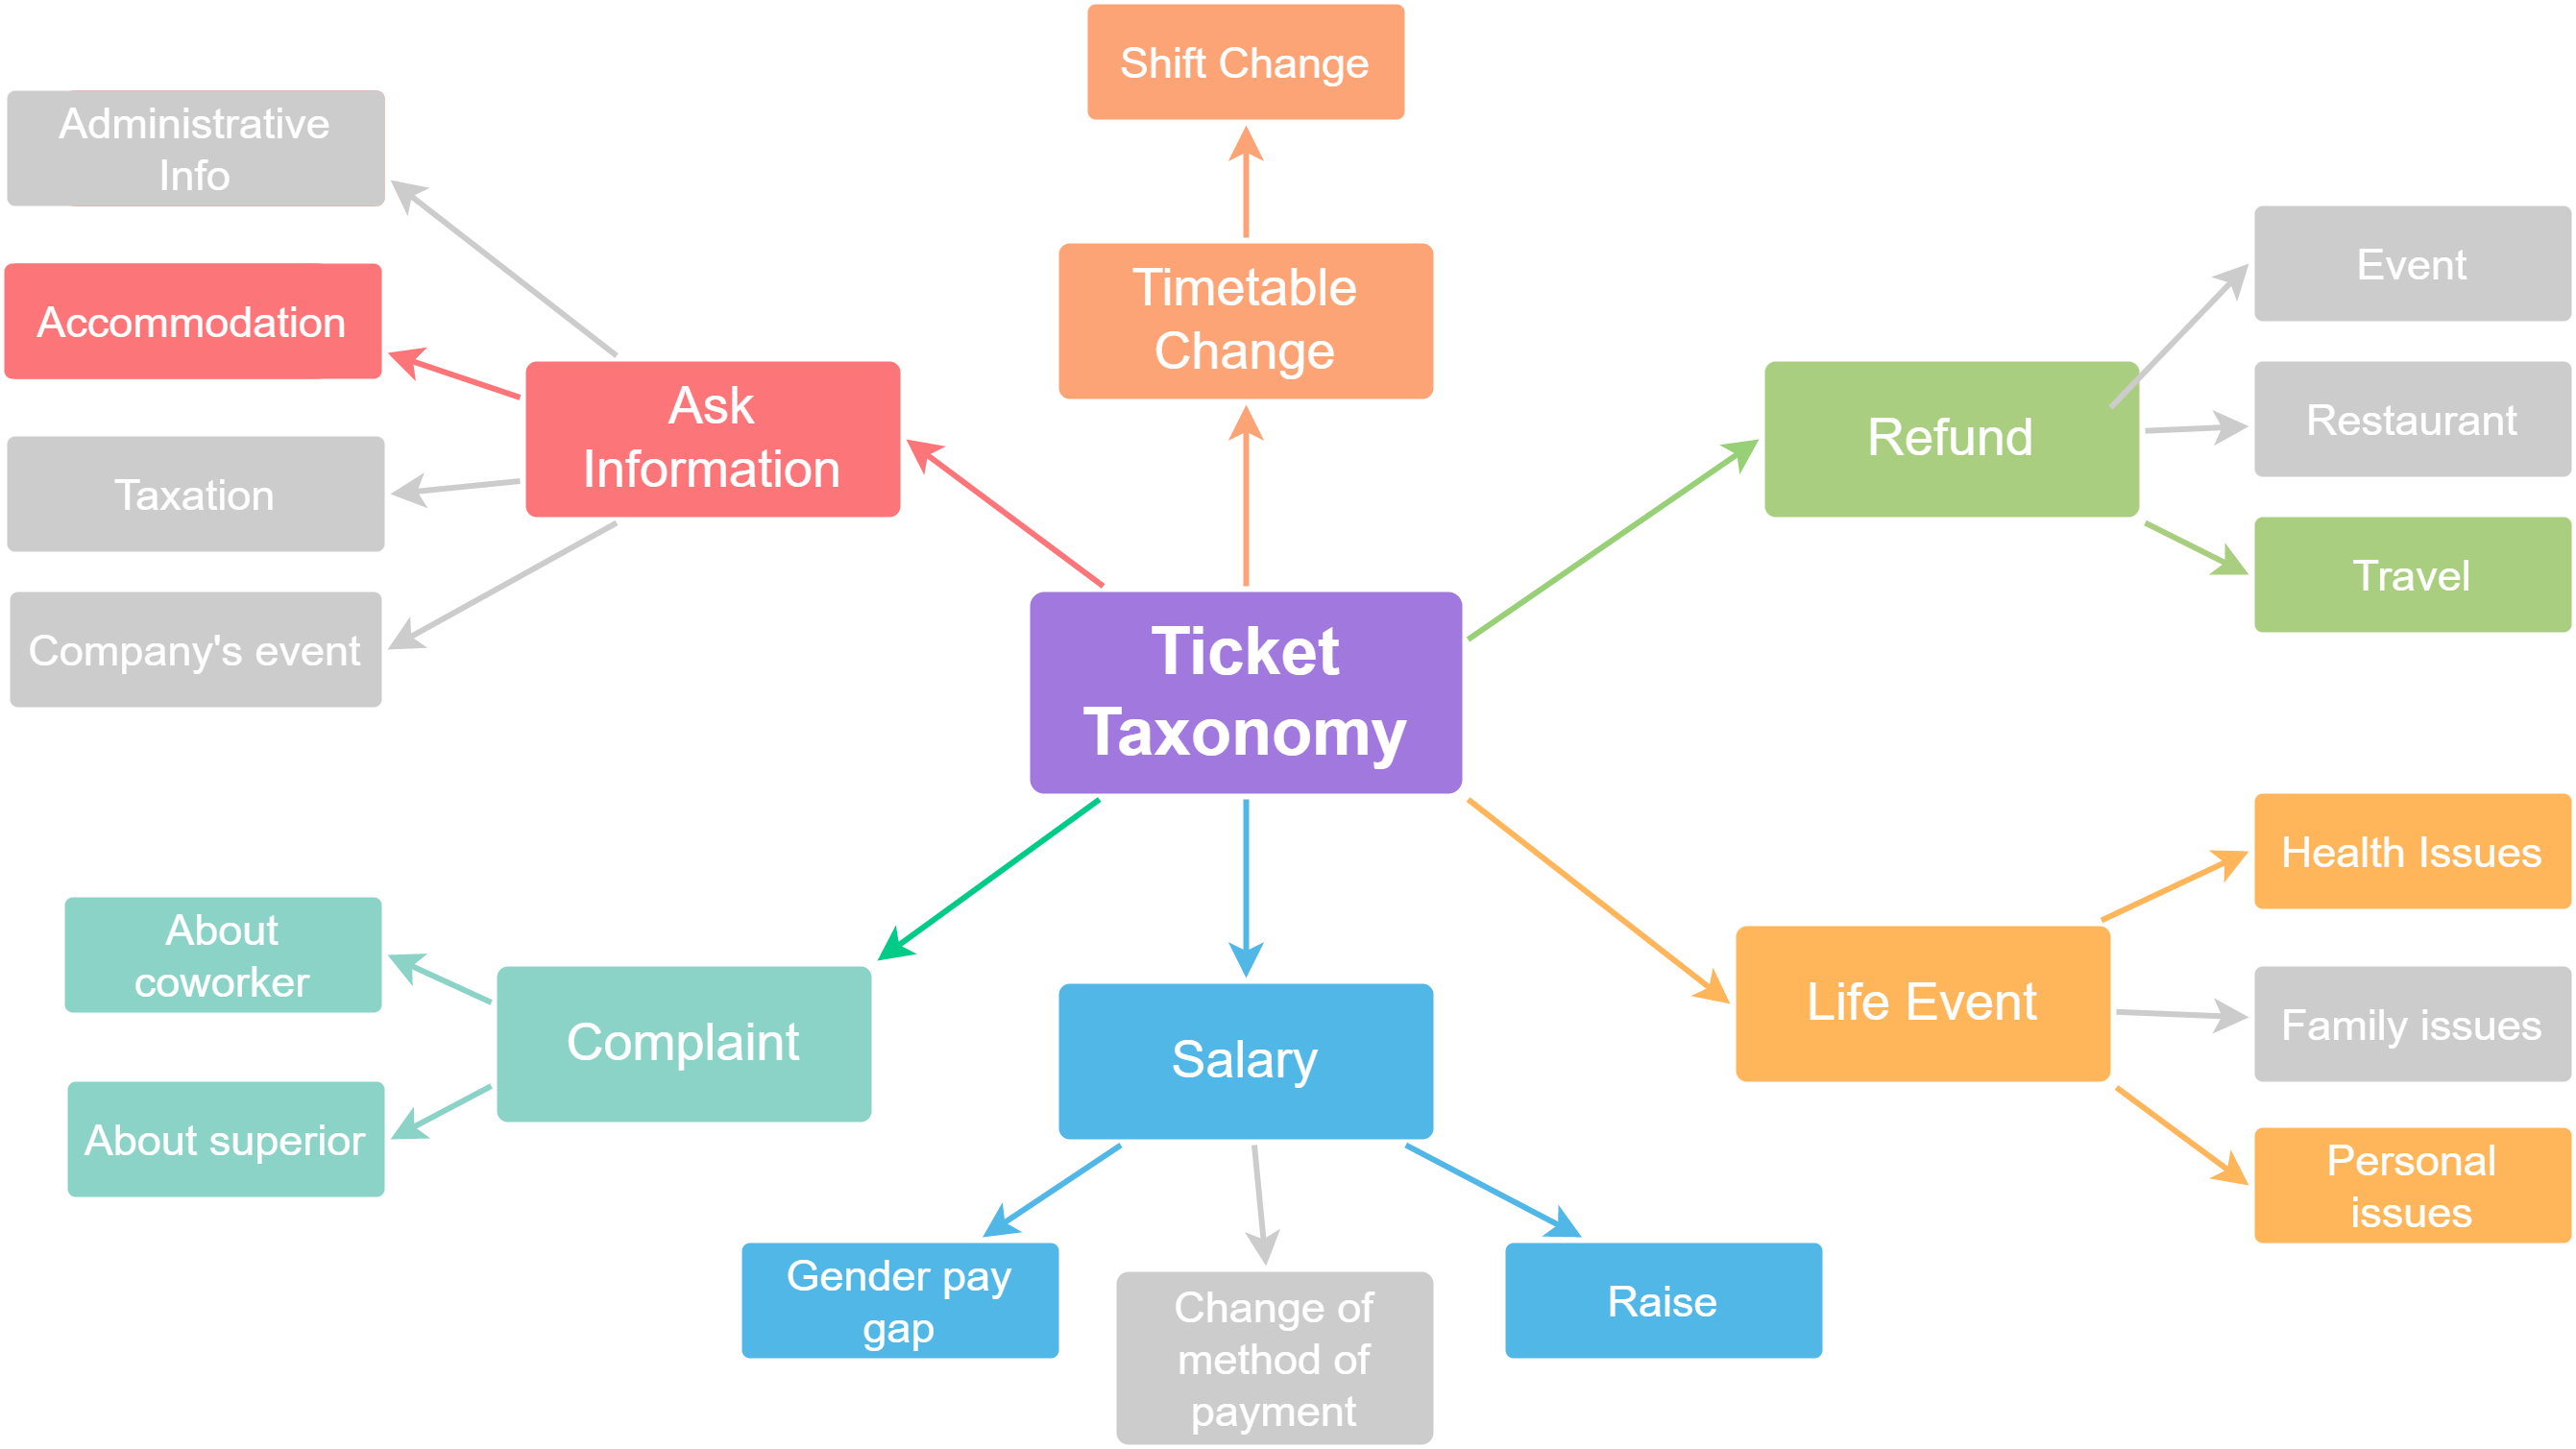
\includegraphics[width=\textwidth]{images/Taxonomy_Tickets_implemented.drawio.png}
    \caption{Final taxonomy, reduced due to unavailability of data}
    \label{fig:final_taxonomy}
\end{figure}    

Usually, HR tickets can belong to various categories, which can range from a request for a shift change to a complaint about a superior. \\
We built a taxonomy of tickets, which is structured into categories and subcategories. Each subcategory has its own variables that are used as inputs for the tickets' generation. The variables are sampled from real-world datasets. \\
For example, to create a request for sick leave, we pass as inputs to our model the reason and the number of days of sick leave requested, which will be acquired from an external dataset. \\
We have a selection of templates and prompts to kick-start the generation process. Every category has its own distinct templates and prompts. The taxonomy (Shown in \autoref{fig:taxonomy} ) has been built following the general structure of the taxonomy of SAP HR tickets, however, the final taxonomy ( Shown in \autoref{fig:final_taxonomy} ) presented here is a subset of the original one due to the unavailability of public data on certain topics ( Ex. \textit{Work benefits}) \\ The final complete taxonomy and the complete list of all variables used for each category/sub-category can be seen in the \autoref{table:categoriesTable}


\begin{table}[h]
    \resizebox{\textwidth}{!}{
    \begin{tabular}{|l|l|l|}
    \hline
        Category            & Sub-category   & variables                                   \\ \hline
        Ask Information     & Accommodation   & location, duration                          \\
        Complaint           & About coworker & complaint, reason                           \\
                            & About superior & complaint, reason                           \\
        Timetable change    & Shift change   & reason\_of\_change, old\_date, new\_date    \\
        Salary              & Salary raise   & old\_salary, new\_salary, increase,work\_title \\
                            & Gender pay gap & wage\_gap                                   \\
        Life Event          & Health issues  & disease, number\_of\_days\_of\_sick\_leave  \\
                            & Personal issues  & issue, number\_of\_days                   \\
        Refund              & Travel         & from, to, date\_travel                     \\
    \hline
    \end{tabular}
    }
\caption{Table of all defined categories and sub-categories with their respective variables}\label{table:categoriesTable}
\end{table}